To prepare this radioactive liquid source, $1.86~\gram$ (uncertainty of $0.05\%$) of tritium was purchased from the Germany company PTB\footnote{Physikalisch-Technische Bundesanstalt, Braunscheweig and Berlin, Germany}, which has a serial number of $2005-1442$ and reference number of PTB-$6.11-285/03.2017$ \cite{TritiumSourceTechnicalFile}

%It had an activity of $26,8 \pm 0.6 ~\mega\becquerel/\gram$ measured with the TRI-CARB 2810 system, based on liquid scintillation readout by PMTs.

The activity of this tritium source is $26,8~\mega\becquerel/\gram$ (uncertainty of $2.24\%$), reference data of 1 of January of 2017, and it was dissolved in $500~\milli\liter$ (uncertainty of $0.05\%$) of ultrapure water, giving 500 ml of tritium water, to which we will call standard solution, with an activity of $100.096~\kilo\becquerel/\gram$ (uncertainty of $2.24\%$), that's, $99.696~\kilo\becquerel/\liter$ (uncertainty of $2.24\%$), which was measured with the TRI-CARB 2810 system, based on liquid scintillation readout by PMT.

Figure \ref{Fig:TritiumPprototypeFillingProcess} shows the filling of the last prototype developed in the TRITIUM project, called TRITIUM-IFIC 2.

\begin{figure}[hbtp]
\centering
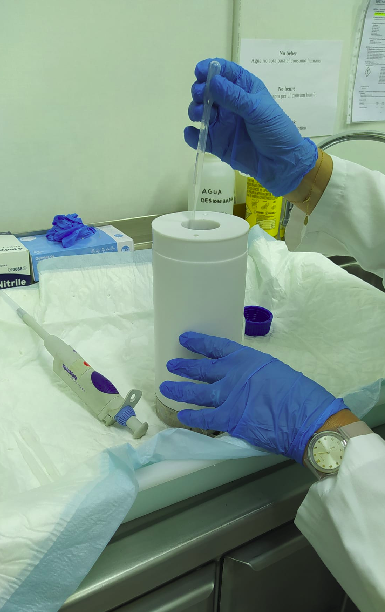
\includegraphics[scale=0.5]{9Appendix/94FillingPrototypes/Filling_TRITIUM_IFIC_2_Prototype.png}
\caption{Filling process of the TRITIUM-IFIC 2 prototype with a tritium water activity of $10~\kilo\becquerel/\liter$\label{Fig:TritiumPprototypeFillingProcess}}
\end{figure}
